\documentclass[a4paper, 10pt]{article}
\usepackage[cm]{fullpage}


\usepackage{listings}
\usepackage{color}

\definecolor{mygreen}{rgb}{0,0.6,0}
\definecolor{mygray}{rgb}{0.5,0.5,0.5}
\definecolor{mymauve}{rgb}{0.58,0,0.82}

\lstset{ %
  backgroundcolor=\color{white},   % choose the background color; you must add \usepackage{color} or \usepackage{xcolor}
  basicstyle=\footnotesize,        % the size of the fonts that are used for the code
  breakatwhitespace=false,         % sets if automatic breaks should only happen at whitespace
  breaklines=true,                 % sets automatic line breaking
  captionpos=b,                    % sets the caption-position to bottom
  commentstyle=\color{mygreen},    % comment style
  deletekeywords={...},            % if you want to delete keywords from the given language
  escapeinside={\%*}{*)},          % if you want to add LaTeX within your code
  extendedchars=true,              % lets you use non-ASCII characters; for 8-bits encodings only, does not work with UTF-8
  frame=single,                    % adds a frame around the code
  keepspaces=true,                 % keeps spaces in text, useful for keeping indentation of code (possibly needs columns=flexible)
  keywordstyle=\color{blue},       % keyword style
  language=Octave,                 % the language of the code
  morekeywords={*,...},            % if you want to add more keywords to the set
  numbers=left,                    % where to put the line-numbers; possible values are (none, left, right)
  numbersep=5pt,                   % how far the line-numbers are from the code
  numberstyle=\tiny\color{mygray}, % the style that is used for the line-numbers
  rulecolor=\color{black},         % if not set, the frame-color may be changed on line-breaks within not-black text (e.g. comments (green here))
  showspaces=false,                % show spaces everywhere adding particular underscores; it overrides 'showstringspaces'
  showstringspaces=false,          % underline spaces within strings only
  showtabs=false,                  % show tabs within strings adding particular underscores
  stepnumber=2,                    % the step between two line-numbers. If it's 1, each line will be numbered
  stringstyle=\color{mymauve},     % string literal style
  tabsize=2,                       % sets default tabsize to 2 spaces
  title=\lstname                   % show the filename of files included with \lstinputlisting; also try caption instead of title
}
\usepackage{graphicx} % Required for the inclusion of images
\usepackage{natbib} % Required to change bibliography style to APA
\usepackage{amsmath} % Required for some math elements 

\setlength\parindent{0pt} % Removes all indentation from paragraphs

\title{Seismic Processing \\ Prac 1 - Building a Synthetic Record.} % Title

\author{ERTH3021} % Author name

\date{\today} % Date for the report

\begin{document}

\maketitle % Insert the title, author and date
This is the first of three pracs on seismic data processing.  This prac is dedicated to building a synthetic 2D seismic dataset. The primary motivation for building a synthetic dataset for processing is to ensure we know what the answer is before we start, and thus can assess the effectiveness of our data processing.  
\par~\\
The second prac will involve building the tools needed to process a seismic dataset.  We will test these tools on the models generated today.
\par~\\
The third prac will use these tools to process a real seismic dataset.

\section{Introduction}

The core concept used to create this synthetic model is known as the convolutional model. The convolutional model states that a recorded signal is the convolution of a source wavelet with the earth's response, convolved with the recorder response, plus some additional noise, i.e.

\[Y(t) =  S(t) * E(t) * R(t) + N(t)\]

where
\begin{itemize}
\item Y(t) is our recorded signal
\item S(t) is the source wavelet
\item E(t) is the earth's response
\item R(t) is the recorder response
\item N(t) is some noise
\item * is the convolutional operator
\end{itemize}

We are going to break the earth's response $E(t)$ into 3 main components - 
\begin{itemize}
\item A(t) - the direct wave
\item B(t) - the refracted wave
\item C(t) - the reflected wave
\end{itemize}

and we are going to ignore the recorder response for this prac.  Thus our synthetic signal can be described as 

\[ Y(t) = \left[ A(t) + B(t) + C(t) \right] * S(t) + N(t) \]

Each component described above will be addressed as a separate exercise.
\par~\\
This prac uses python as a teaching tool.  The entire prac consists of several hundred lines of code. A significant proportion of this code has been supplied.  This supplied code uses some advanced processing techniques, for example classes and decorators.  The main reason for this is to reduce the amount of boilerplate code.  Understanding this part of the code  is not required for this prac.  
\par~\\
The assessment of this prac will take the form of a brief report.  This report should include a summary of the main components of the prac (suggested with an asterisk), as well as screen shots from each exercise.  A brief paragraph and/or bullet points which shows understanding of the major concepts is sufficient.  

\section*{Exercise 1 - Initial Setup}
\begin{enumerate}
\item *Load and view earth model
\item Initialise parameter dictionary
\item Initialise data workspace
\item *Define survey geometry
\item Load initialisation values
\item *Write test signal
\item *View result.
\end{enumerate}


\section*{Exercise 2: Direct Wave}
The direct wave travels along the earth/air interface, and can thus be calculated from the velocity formula

\[ v = \frac{s}{t} \]

where 
\begin{itemize}
\item v = velocity
\item s = displacement
\item t = time
\end{itemize}

Spherical divergence is the idea that as a wave spreads out, the energy in the wave spreads out over the surface of the waveform. The amplitude of the wave is inversely proportional to the square of the distance traveled, i.e.

\[ A = \frac{1}{distance^2}\]

\begin{enumerate}
\item *Create a function which calculates the direct travel time, given a velocity and distance
\item *Create a function which calculates the spherical divergence weighting, given a distance
\item Apply weights to traveltimes
\item Write valid results to workspace
\item Display Result
\item Apply AGC
\item *Display result with AGC
\end{enumerate}

\newpage
\section*{Exercise 3: Refracted Wave}
\begin{figure}[h]
\centering
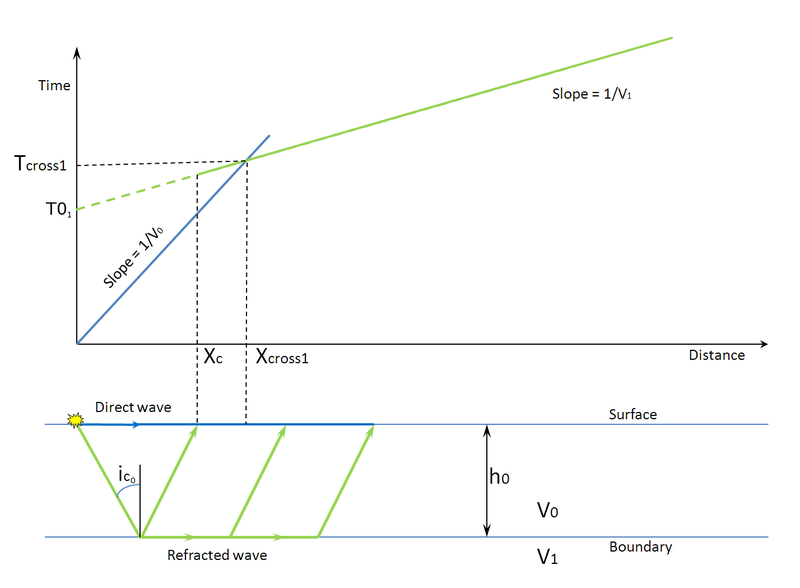
\includegraphics[scale=0.5]{800px-Refraction_2layers.png}
\caption{Calculating refraction travel-time, image from wikipedia}
\end{figure}
The formula to calculate the refracted travel time is 
\[T = \frac{X}{V_1} + \frac{2z \cos{i_c}}{V_0}, \quad i_c = \sin^{-1}{\frac{V_0}{V_1}} \]
Where
\begin{itemize}
\item $X$ = lateral distance
\item $V_0$ = velocity of weathering layer
\item $V_1$ = velocity of sub-weathering layer
\item $z$ = thickness of weathering layer
\item $i_c$ = critical angle
\end{itemize}

The exercise consists of the following steps:

\begin{enumerate}
\item *Create a function which calculates the refracted travel time
\item Apply spherical divergence to travel times
\item Write valid results to dataset
\item *Display result
\end{enumerate}

\newpage
\section*{Exercise 4: Reflected Wave}
\begin{figure}[h]
\centering
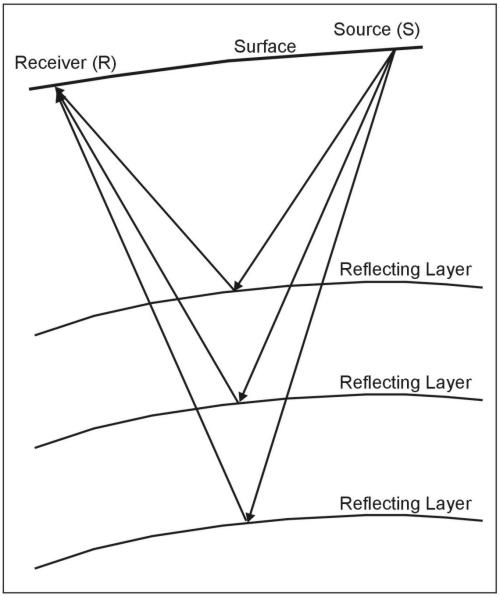
\includegraphics[scale=2.0]{reflection.jpg}
\caption{Calculating reflection travel-time, image from the U.S. EPA website}
\end{figure}

Calculating the reflection times in a homogeneous earth is relatively simple.  Calculating the travel time in an inhomogeneous earth is less simple.  Functions have been provided which will perform most of the hard lifting for this.
\par~\\
Calculating amplitudes can also be complex.  A relatively accurate approximation might involve the Aki-Richards equations seen on the Crewes Zeoppritz Explorer.  Instead, for this exercise,  we will use the zero-offset reflection and transmission coefficients.

\[ R_r = \frac{z_1 - z_0}{z_1+z_0}\]
\[ R_t = \frac{2*z_0}{z_1+z_0}\]

where 
\begin{itemize}
\item $z_0$  = acoustic contrast in layer 0, i.e. $\rho_0 v_0$
\item $z_1$ = acoustic contrast in layer 1, i.e. $\rho_1 v_1$
\end{itemize}

This exercise will include the following steps:


\begin{enumerate}
\item *Implement functions to calculate reflection and transmission coefficients
\item *Discuss geometry of calculations
\item Calculate reflection traveltimes (using supplied point extrapolation routine)
\item Calculate transmission amplitudes (using supplied point extrapolation routine)
\item Calculate reflection amplitudes
\item Write result to dataset
\item *Display Result
\end{enumerate}


\section*{Exercise 5: Build Combined Shot-record}

\begin{enumerate}
\item *Write function which combines exercises 2, 3 \& 4.
\item *Convolve with wavelet
\item *Display result
\item *Add noise
\item *Display result
\end{enumerate}
\section*{Exercise 6: Exploring Advanced Modelling Techinques}

This exercise examines alternative modelling techniques, including finite difference modelling and bent-ray ray-tracing.

%\newpage
%\lstinputlisting{../exersize1.py}
%\lstinputlisting{../exersize2.py}
%\lstinputlisting{../exersize3.py}
%\lstinputlisting{../exersize4.py}
%\lstinputlisting{../exersize5.py}
%\lstinputlisting{../exersize6.py}

\end{document}